\chapter[Visão do Produto]{Visão do Produto}

\section{Visão Estrutural}

Ao desenhar a estrutura do Robô foi identificado que deve-se levar em consideração os seguintes aspectos:
\begin{enumerate}
	\item Melhor identificação da criança com o equipamento
	\item Segurança
\end{enumerate}

Melhor identificação da criança com o equipamento:
\begin{itemize}
\item Cor: Pagnan, C. M. et al afirma que a cor exerce uma ação tríplice: a de impressionar a de expressar e a de construir, portanto o aparelho deve apresentar coloração atrativa para a criança, e também faz uma relação entre as cores e as respectivas características psicológicas e simbólicas, para os propósitos do trabalho selecionamos duas cores:
\item Azul: Exerce apelo intelectual, simbolizando a inteligência e raciocínio.
\item Vermelho: Estimulante e dinâmica é a cor preferida da criança.
\item Aparência: Quanto a aparência ela deve ter aparência agradável, intuitiva e associado a elementos que o usuário conheça e se identifique, as formas especuladas são veículos e elementos de filmes desenhos e etc.
\end{itemize}

\textbf{Segurança}:
O produto oferecido não deve apresentar nenhum tipo de risco a integridade física da criança, portanto o produto deve possuir design “macio”, não apresentando pontas ou qualquer componente que venha a amplificar um possível tipo de dano causado por contato mecânico.

\textbf{Design}:
A estrutura foi desenhada no software CATIA, o intuito foi lembrar a estrutura de um carrinho, elemento a qual a criança já está acostumada. Alguns elementos como iluminação a led e desenhos vão ser introduzidos na estrutura física final de modo a tornar o carrinho ainda mais atrativo para a criança.

\begin{figure}[H]
    \centering
    
\includegraphics[width=0.8\textwidth]{figuras/estrutura_catia.eps}
    \caption{}
    \label{fig:catia01}
\end{figure}

\textbf{Peso}: Ao realizar o assembly das peças no CATIA utilizou –se uma ferramenta no próprio software para estimar o peso do carrinho, o valor obtido foi de aproximadamente 3,5 Kg. Porem como faltou o cad de alguns dos componentes o valor da massa utilizado nos demais cálculos foi de 4 Kg para contabilizar eses componentes e oferecer uma certa margem de erro.


- \textbf{Materiais}:
Para selecionarmos o material a ser utilizado na estrutura os critérios considerados foram:
\begin{itemize}
\item Segurança
\item Propriedades mecânicas
\item Proteção dos equipamentos eletrônicos
\end{itemize}

Inicialmente foi considerado a escolha de dois tipos de materiais o alumínio e polímeros.
 
Segurança da criança: Nesse aspecto os riscos identificados foram:
\begin{enumerate}
\item Toxicidade
\item Choques mecânicos
\end{enumerate}

Segundo a Ficha de informações de segurança do produto químico da The Dow Chemical Company o HDPE não é uma Substância Química Perigosa, classificado pela definição do Padrão OSHA de Comunicação de Perigos, 29 CFR 1910.1200. Ainda segunda a The Dow Chemical Company o contato prolongado não é irritante para a pele e nem a pele absolve de alguma maneira o material, portanto os principais riscos que o material deve apresentar são inerentes a todos os materiais e se devem a choques mecânicos. Esses choques mecânicos podem ser amenizados dependendo do processo de fabricação, que pode ser escolhido para produzir um material mais ‘macio’ e que ao mesmo tempo aguente os esforços mecânicos a qual o robô será submetido.

Propriedades mecânicas: Os principais esforços identificados a qual o robô será submetido foram:
\begin{enumerate}
\item Queda
\item Peso (devido a objetos em cima do robô)
\item Choques com obstáculos
\end{enumerate}

\begin{figure}[H]
    \centering
    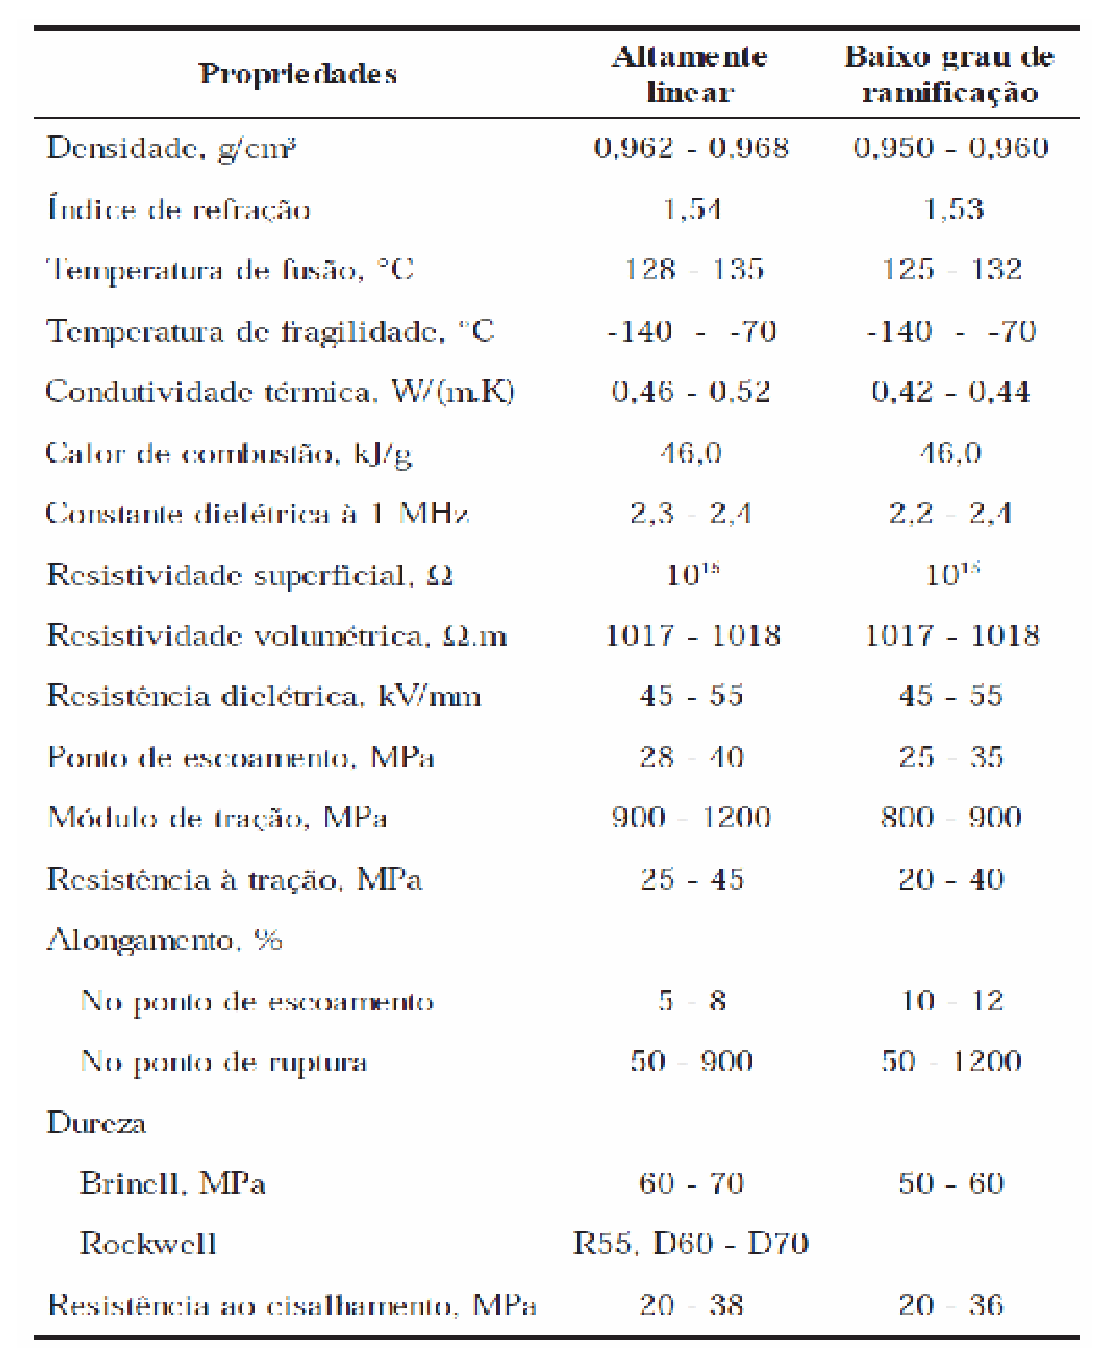
\includegraphics[width=0.8\textwidth]{figuras/tabela_pead.eps}
    \caption{}
    \label{fig:catia01}
\end{figure}

Em comparação com o alumínio que foi o outro material considerado que é comumente usado nesse tipo de aplicação, essas propriedades validam o uso do HDPE no projeto. O grande diferencial do HDPE foi o preço e a maior facilidade de conformar o material para forma desejada. Segue abaixo uma tabela com as propriedades do alumínio CAST 7000, um dos mais usados para construção de chassi de maquinas no geral:

Proteção dos equipamentos eletrônicos: Nesse tópico as principais preocupações foram:
\begin{enumerate}
\item Transferência de calor.
\item Condução elétrica.
\end{enumerate}

Como podemos ver, o HDPE apresenta as propriedades de condução térmica e elétrica em ordens de grandeza bem menor que a do alumínio. Portanto é o mais indicado nesse quesito.

De todos os 3 aspectos considerado o HDPE apresenta um maior número de vantagens em todos, no quesito das propriedades mecânicas embora o alumínio ofereça propriedades mecânicas superiores, esses valores estão muito acima da necessidade do projeto, logo o HDPE foi o material selecionado para desenvolvermos o chassi do robô.
 
\textbf{Analise Estrutural}

A análise estrutural foi realizada no software ASYNS e foi feita apenas para o caso estático. No caso dinâmico, o software recebe os parâmetros físicos do carrinho e as condições de contorno que seria a de uma free wall, ao final da simulação o software retorna os valores dos parâmetros em um intervalo de tempo. Esse tipo de simulação é muito complexa e geralmente requer grande poder de processamento. O caso estático funciona de maneira semelhante porem as condições de contorno são diferente e o resultado é valido apenas para uma unidade de tempo, nesse tipo de simulação deve ser feita uma análise antes de maneira a obter os resultados no tempo certo.

Os parâmetros analisados foram a deformação que a estrutura sofre, e a tensão de Von Mises que é um critério utilizado para prever a falha de materiais frágeis.

\textbf{Queda}: no caso da queda a unidade de tempo desejada é a que a magnitude da força atuando sobre o carrinho seja a maior possível. As condições de contorno são: um lado do carrinho sem sofrer deslocamento estrutural (deformação) e em algum outro lado aleatório (foi testado em todos os lados) aplica-se uma força igual a força atuante na hora do impacto:

\textbf{Deformação}:

\begin{figure}[H]
    \centering
    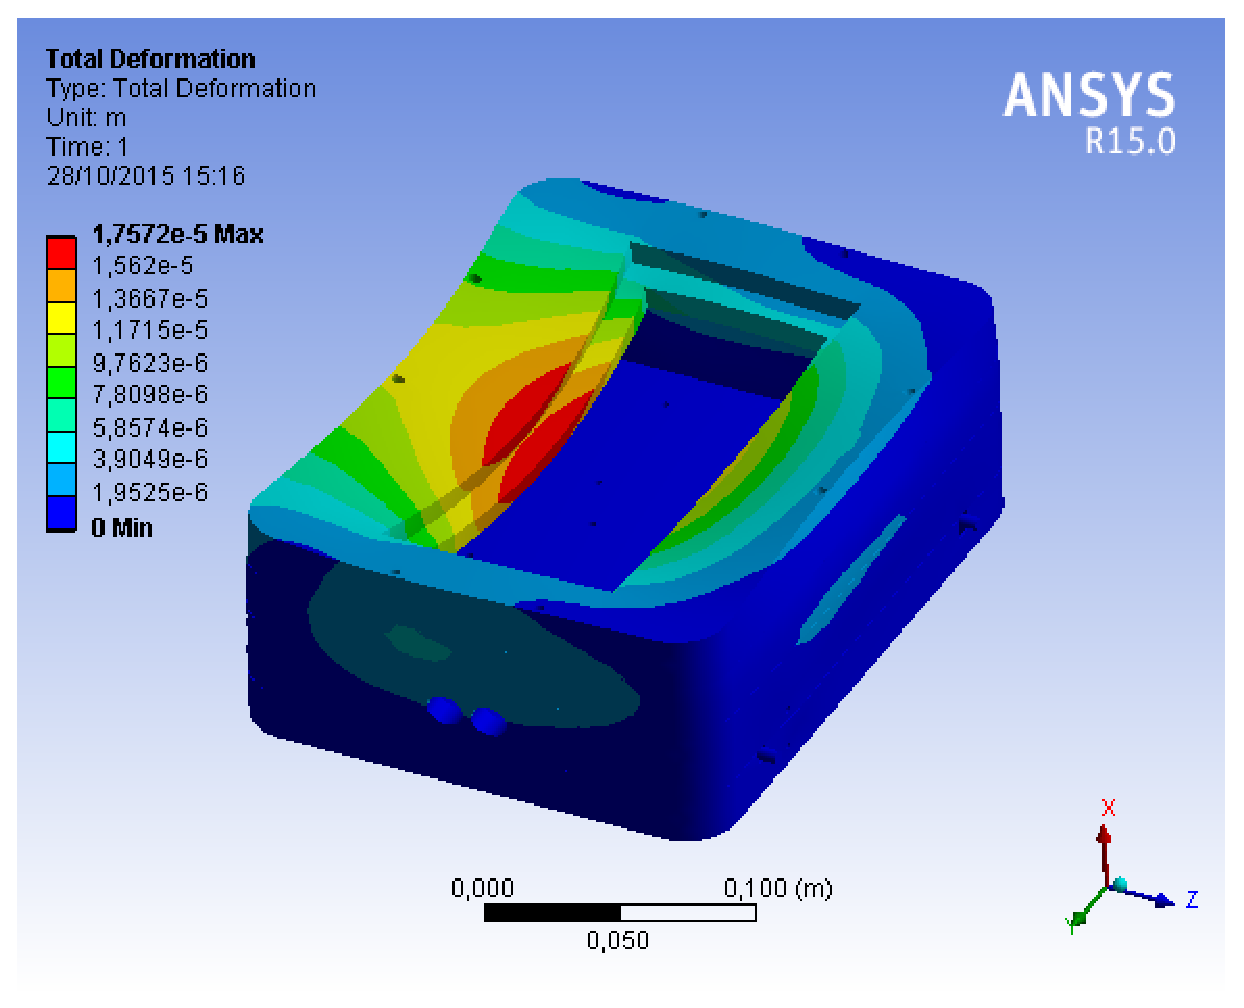
\includegraphics[width=0.8\textwidth]{figuras/deformacao_1000n.eps}
    \caption{}
    \label{fig:catia01}
\end{figure}

\begin{figure}[H]
    \centering
    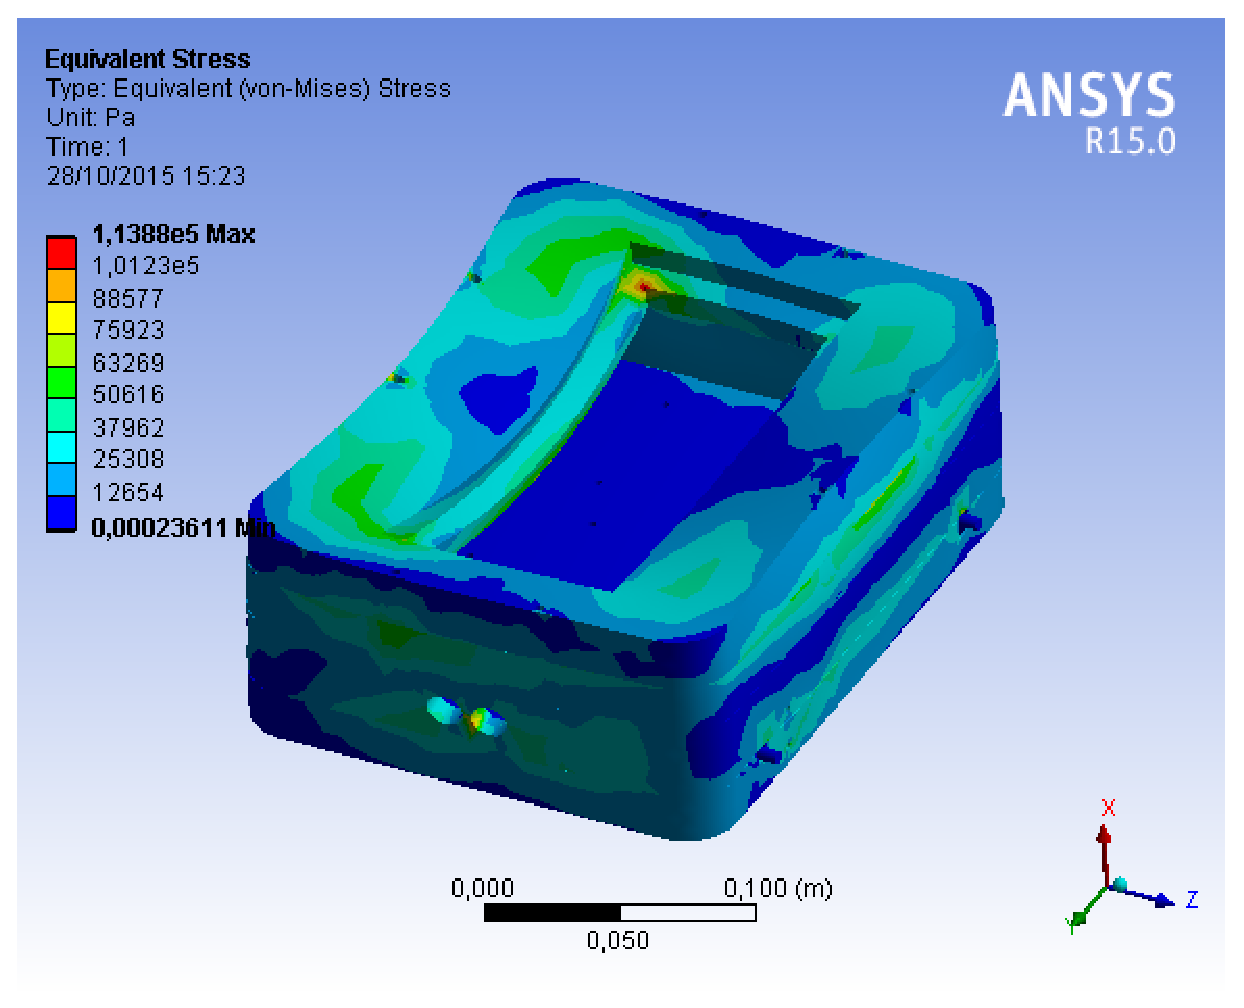
\includegraphics[width=0.8\textwidth]{figuras/vonmises_1000n.eps}
    \caption{}
    \label{fig:catia01}
\end{figure}

Nas ilustrações acima as condições de contorno são: Força de 1000 N (valor super estimado pela interação ser de impacto) na face superior, força de 50 N na face lateral, a face inferior e os eixos fixos. Como podemos ver não ocorre nenhum deslocamento exagerado e a superfície permanece a praticamente a mesma com o maior deslocamento sendo da ordem de 10e-5 m. Na análise do critério de Von Mises o maior valor atingido é de 113,8 KPa o que é menor que os valores de ruptura dos materiais utilizados  na ordem de 10e3.
 
\textbf{Sobrepeso}: O caso estático fornece uma excelente resultado para o sobrepeso do carrinho, pois estamos analizando a estrutura com o peso já em cima não o comportamento da estrutura ao impacto do peso. As condições de contorno usadas na análise foram: Força de 100 N na parte superior do carrinho, eixos e parte inferior fixa (parte que não se move).
 
\textbf{Deformação}:

IMG

IMG

Como podemos ver o valor máximo da deformação é da ordem de 10e-5m o que significa que nessas condições não ocorre uma deformação expressiva no carrinho. Os valores da tensão de Von Mises não apresentam valores que possam oferecer um real risco a integridade do material pois apresentam valores da ordem de 10e3 menores que o valor da tensão de ruptura do material.
 
Choque com obstáculos: A velocidade do carrinho é relativamente baixa, em um impacto a magnitude das forças envolvidas são bem menores do que a magnitude das forças atuando na queda, como a simulação da queda validou a estrutura do carrinho estendemos os resultados para a análise de colisões e afirmamos que a estrutura desenvolvida está apta a colidir nas condições normais de operação do carrinho.
 
Como a estrutura desenvolvida não apresentou problemas em nenhum dos casos simulado, podemos afirmar que a estrutura cumpre os requisitos do projeto e portanto o seu uso é valido.

\subsection{Atuadores}

Os atuadores são os componentes que convertem a energia em potência mecânica, no caso em questão utilizaremos uma bateria para alimentação do alfa. Por meio de conversão eletromecânica a energia elétrica é convertida em potência mecânica e enviada para os elos, responsáveis pela movimentação do alfa.  Os atuadores utilizados em robôs de modo geral, são os atuadores eletromagnéticos, principalmente os que utilizam motores de corrente contínua e de passo. Os motores elétricos são interessantes no projeto de robôs, devido ao fato de que estes quando associado a sensores possibilitam tanto o controle de força quanto de posicionamento do robô, a facilidade na programação dos seus movimentos, visto que são controlados por sinais elétricos, até a utilização de controladores de movimentos (ROMANO \& DUTRA, 2002).

Os motores elétricos são divididos basicamente em: motores de corrente alternada (ca/ac) e motores de corrente continua (cc/dc). Os motores de corrente alternada são vantajosos devido a sua construção ser bastante simples, e a sua alimentação ocorrer diretamente da rede. No entanto nos projetos na área da robótica os motores de corrente contínua são os mais utilizados, devido a alimentação nestes tipos de projeto ocorrem na sua grande maioria a partir de bateria, as quais funcionam com corrente contínua, com isso a utilização de inversores não se faz necessária (BRAGA, 2006).


Além da alimentação dos motores de corrente contínua, outras vantagens em sua utilização, são devido: (BRAGA, 2006).
\begin{itemize}
\item a velocidade do motor ser ajustada a partir de um potenciômetro, realizando a variação da tentão aplicada sobre o motor;
\item o sentido de rotação do motor pode ser alterado a partir da alteração da polaridade da tensão aplicada ao motor;
\item ao controle da aceleração e desaceleração do motor promovendo uma resposta no tempo ou para suavizar o funcionamento deste;
\item a possibilidade de controle do torque a partir da variação da corrente aplicada no motor;
\item a apresentarem uma resposta rápida, ou seja, quando submetidos a voltagens elevadas acelera rapidamente.
\end{itemize}

Os motores utilizado no alfa são motores dc, com caixa de redução 1:48, e eixo duplo, a escolha desse motor ocorreu devido aos fatores apresentados acima. Abaixo será apresentado uma tabela com as especificações do motor que será utilizado.

IMG

IMG

\subsection{Alimentação}

A alimentação dos componentes será feita por intermédio da placa Raspberry pi, o levantamento das necessidades energéticas delimitou que a placa necessita de uma tensão constante em 5 volts, recebendo 2 ampères de corrente.  Assim surgiram duas opções de alimentação: Pilhas ou Baterias.

As pilhas podem ser divididas em recarregáveis e não recarregáveis. As pilhas recarregáveis apesar de mais caras, possuem a vantagem de serem usadas em centenas de ciclos de carga e recarga. As de uso único tornam o projeto mais barato, entretanto o custo de troca de pilhas reaparece várias vezes para o consumidor. Independentemente do tipo de pilha utilizada, as pilhas comerciais apresentam valores de tensão e corrente muito abaixo do necessário, sendo necessário colocar várias em série para elevar a tensão e várias em paralelo, para elevar a corrente de alimentação. Isso acaba tornando o uso de pilhas nada prático.

Além de que a tensão de pilhas cai de acordo com a capacidade é utilizada, fazendo com que a placa desligasse antes da pilha estar totalmente carregada pelo fato da tensão não estar adequada, a figura abaixo ilustra (para uma pilha AA “heavy duty”).

IMG

As baterias encontradas no mercado podem ser de vários tipos, as mais comuns são as de Ion-Lítio, a maior vantagem delas é o seu fator energético em função do peso ser alto, elas costumam ser bem mais leves que outras baterias recarregáveis de mesmo tamanho (geralmente 150 watt-hora para cada quilo de bateria), além de serem bem mais baratas e seguras que outras baterias, como as de chumbo-ácido.

A bateria escolhida é a KMASHI MP816, por apresentar uma capacidade nominal de 10 Ah, atendendo ao projeto. Sua recarga é rápida e sua descarga pode ser controlada de acordo com a necessidade do projeto.  Para verificar se a carga real era próxima da nominal, um teste de carga foi realizado. O peso da bateria é de 280 gramas.

Ao se manter uma tensão constante de 5V e 2A (totalizando 10W de potência nominal para recarga) a bateria necessitou de em média 3 horas para atingir uma carga satisfatória (90\% da carga), em uma alimentação forçada de 4 horas, o nível de carga subiu pouco (em torno de 5\%) comparado às 3 horas iniciais. Logo o sistema possui um tempo de recarga para valores satisfatórios de 3 horas quando se utiliza uma fonte D.C. de 10 watts de potência. Para a descarga, o sistema apresenta um valor um pouco inferior. 2 horas e 50 minutos de autonomia em média, considerando que a carga será constante de 10,5 watts.

\subsection{Giro e Curvas}

Quando for enviado o sinal para que o carrinho gire para a direita e para a esquerda, um dos motores será desligado assim com a força do único motor ligado as duas rodas frontais acompanham a roda que está sendo estimulada pelo motor e auxiliam para que o robô complete o giro, dessa forma obedecendo o comando, (o motor que será desligado dependerá do sentido que o robô irá se mover.
 
O princípio de usar esteiras neste carrinho é que este poderá passar por locais em que o piso não é plano, sendo assim para o bom funcionamento das mesmas o carrinho terá dois motores  para mover as esteiras da direita e da esquerda independentes. 

\section{Visão e Controle e Processamento}

Segue um diagrama de sequência com a visão geral de como o robô Alfa irá funcionar e da comunicação entre os sistemas:

IMG

\subsection{Aplicativo}
O aplicativo de controle do robô será implementada para o sistema operacional Android usando a linguagem de programação Java. A versão mínima do SDK será a 8 e a versão alvo será a 23. Por tanto as versões do SO suportadas serão da 2.2 (Froyo) até a 6.0 (Marshmallow).

Os métodos que merecem destaque são MyTouchListener() e a função de criação e envio das instruções:
\begin{itemize}
\item MyTouchListener(): responsável pelo monitoramento dos toques na tela do usuário. Implementada a partir da interface View.OnTouchListener
\item Função de criação e envio das instruções: após o usuário ordenar as instruções para o robô, essa função irá criar um arquivo JSON e enviar as instruções pela conexão WiFi via Socket.
\end{itemize}

As instruções estarão em arquivo JSON, criado no java a partir de JSONObject. Um exemplo de arquivo com as instruções é mostrado na figura abaixo:

Os dados que esse arquivo irá enviar ao Raspberry Pi serão:
\begin{itemize}
\item [IDENTIFICADOR] Comando/instrução: comando ou instrução para o robô, por exemplo vire a direita.
\end{itemize}

Dentro de cada comando/instrução os seguintes campos estão presentes:
\begin{itemize}
\item Position: posição em que determinada instrução está em todo o conjunto de blocos de instruções
\item Duration: no caso de “mover para frente”, será passada o tempo desse movimento. Cada tempo já é determinado: 1, 2, 5, 10. Cada uma dessas instruções será um bloco diferente na interface do aplicativo
\item Degree: são os graus com que o robô irá virar, caso seja necessário (ainda em avaliação).
\item Power: informação ainda em avaliação se será necessária para o robô, dado que todo o sistema de hardware e mecânico já está definido e não cabe ao aplicativo informar quanto de potência que o motor ou sensor deve ter.
\end{itemize}

Os outros blocos de instrução desejáveis na aplicação, a saber o de obstáculo para introdução do conceito das estruturas de condição e os círculos para introduzir os conceitos de laços de repetição ainda estão em desenvolvimento.